\chapter{O2 module}
\label{subs:O2:mod}

The O$_2$ module is a simple model that describes the oxygen density evolution in the water.
It is activated by setting \telkey{WATER QUALITY PROCESS} = 2.
It offers the advantage of being simple and then easy to calibrate.
Indeed, since some important parameters are kept constant
(such as vegetal respiration \telkey{VEGETAL RESPIRATION R},
benthic demand \telkey{BENTHIC DEMAND}),
only 8 parameters have to be introduced (and, if necessary calibrated).
The use of this module is, consequently, recommended for short time periods (several days).

O$_2$ module uses 3 tracers:

\begin{enumerate}
\item dissolved oxygen O$_2$ (mgO$_2$/l),
\item organic load L (mgO$_2$/l),
\item ammoniacal load NH$_4$ (mgO$_2$/l).
\end{enumerate}

These tracers are hence, advected and dispersed in the whole water mass
and their evolution obeys the advection-diffusion equation linked to external and internal source terms.

For more details about the theory of the O$_2$ module,
the reader can refer to the \waqtel technical manual.


\section{The dissolved oxygen}

The dissolved oxygen density is influenced by the following factors:

\begin{itemize}
\item 4 factors consuming oxygen:

\begin{enumerate}
\item organic load L,
\item ammoniacal load,
\item benthic demand,
\item vegetal respiration,
\end{enumerate}

\item 2 factors producing oxygen
\begin{enumerate}
\item photosynthesis,

\item reaeration.
\end{enumerate}
\end{itemize}
We will introduce briefly how the source terms linked to these six factors are estimated.


\subsection{The benthic demand}

The benthic demand $BEN$ is provided by 
using the keyword \telkey{BENTHIC DEMAND} (default = 0.1~gO$_2$/m$^2$/d).
It is then corrected with water temperature $T$ like:
\[{BEN}_T={BEN}_{20^\circ C}{\left(1.065\right)}^{T-20}\]
Where $T$ is given in $^{\circ}$C using the keyword \telkey{WATER TEMPERATURE}
(default = 7$^\circ$C).
This value of temperature is useful when the temperature is not considered
as a tracer in the model.
Otherwise, the real temperature is taken into account.

The following Table gives some typical values of benthic demand
at $T$ = 20$^\circ$C (i.e. $BEN_{20^\circ \rm{C}}$).\\

\begin{table}[H]
 			\centering
\begin{tabular}{p{3.0in}p{3.0in}}
\hline
%row no:1
\multicolumn{1}{|p{3.0in}}{Bottom type} & 
\multicolumn{1}{|p{3.0in}|}{Typical value of $BEN$ (gO$_2$/m$^2$/d) at 20$^{\circ}$C} \\
\hline
%\hhline{--}
%row no:2
\multicolumn{1}{|p{3.0in}}{Filamentous bacteria (10~g/m$^2$)} & 
\multicolumn{1}{|p{3.0in}|}{7} \\
\hline
%\hhline{--}
%row no:3
\multicolumn{1}{|p{3.0in}}{Mud from waste water, near to release} & 
\multicolumn{1}{|p{3.0in}|}{4} \\
\hline
%\hhline{--}
%row no:4
\multicolumn{1}{|p{3.0in}}{Mud from waste water, far from release } & 
\multicolumn{1}{|p{3.0in}|}{1.5} \\
\hline
%\hhline{--}
%row no:5
\multicolumn{1}{|p{3.0in}}{Estuarine silt} & 
\multicolumn{1}{|p{3.0in}|}{1.5} \\
\hline
%\hhline{--}
%row no:6
\multicolumn{1}{|p{3.0in}}{Sand} & 
\multicolumn{1}{|p{3.0in}|}{0.5} \\
\hline
%\hhline{--}
%row no:7
\multicolumn{1}{|p{3.0in}}{Mineral soil} & 
\multicolumn{1}{|p{3.0in}|}{0.007} \\
\hline
%\hhline{--}

\end{tabular}
\end{table}


\subsection{Vegetal respiration}

It is given directly by the user with keyword \telkey{VEGETAL RESPIRATION R}
(default = 0.06~mgO$_2$/d/l).


\subsection{Photosynthesis P}

The photosynthesis $P$ depends on algae density,
water depth and sunlight,
with order of magnitude between 0.3 and 9 mgO$_2$/d/l.
For O$_2$ module, $P$ is given by the user with the keyword
\telkey{PHOTOSYNTHESIS P} (default = 1~mgO$_2$/d/l).


\subsection{Reaeration}

It is the gain oxygen through the free surface of water.
It is due to 2 main reasons:
\begin{itemize}
\item the natural reaeration,
\item the weir reaeration.
\end{itemize}

\subsubsection{Natural reaeration}
It can be seen at a macroscopic level
as a term which is linearly dependent on ($C_s-[O_2]$),
where $C_s$ is O$_2$ saturation density of water
(given through keyword \telkey{O2 SATURATION DENSITY OF WATER (CS)},
default = 11~mg/l) and [O$_2$] is the O$_2$ density.
For instance $C_S$ = 9~mg/l at 20$^\circ$C.
We get finally:

\begin{equation*}
Natural~reaeration = k_2(C_S-[O_2]),
\end{equation*}

where $k_2$ (given in d$^{-1}$) is an empirical parameter
which can be computed using 4 empirical laws.

Its orders of magnitude are indicated in the Table below
(from \cite{tchobanoglous_wq_1985}).\\

\begin{table}[H]
 			\centering
\begin{tabular}{p{3.0in}p{3.0in}}
\hline
%row no:1
\multicolumn{1}{|p{3.0in}}{Type of watercourse} & 
\multicolumn{1}{|p{3.0in}|}{Interval of $k_2$ (d$^{-1}$) at 20$^{\circ}$C} \\
\hline
%\hhline{--}
%row no:2
\multicolumn{1}{|p{3.0in}}{Small ponds and backwaters} & 
\multicolumn{1}{|p{3.0in}|}{0.10-0.23} \\
\hline
%\hhline{--}
%row no:3
\multicolumn{1}{|p{3.0in}}{Sluggish streams and large lakes} & 
\multicolumn{1}{|p{3.0in}|}{0.23-0.35} \\
\hline
%\hhline{--}
%row no:4
\multicolumn{1}{|p{3.0in}}{Large streams of low velocity flow} & 
\multicolumn{1}{|p{3.0in}|}{0.35-0.46} \\
\hline
%\hhline{--}
%row no:5
\multicolumn{1}{|p{3.0in}}{Large streams of normal velocity flow} & 
\multicolumn{1}{|p{3.0in}|}{0.46-0.69} \\
\hline
%\hhline{--}
%row no:6
\multicolumn{1}{|p{3.0in}}{Swift streams} & 
\multicolumn{1}{|p{3.0in}|}{0.69-1.15} \\
\hline
%\hhline{--}
%row no:7
\multicolumn{1}{|p{3.0in}}{Rapids and waterfalls} & 
\multicolumn{1}{|p{3.0in}|}{> 1.15} \\
\hline
%\hhline{--}

\end{tabular}
\end{table}

The choice of the law is given by the keyword
\telkey{FORMULA FOR COMPUTING K2} which can have the following values:

\begin{itemize}
\item 0: $k_2$ constant (default formula), its value is given by keyword
  \telkey{K2 REAERATION COEFFICIENT} (default = 0.9~d$^{-1}$),
\item 1: formula of the Tenessee Valley Authority,
  %: $k_2 = 5.23\ U.h^{-1.67}$
  %with $U$ is the velocity
  %and $h$ is the water depth at each point of the mesh
\item 2: formula of Owens et al.,
  %$k_2 = 5.33\ U^{0.67}h^{-1.85}$
\item 3: formula of Churchill et al.,
  %$k_2 = 0.746\ U^{2.695}h^{-3.085}J^{-0.823}$
  %where $J$ is the head loss .
\item 4: formula of O'Connor \& Dobbins,
  %$k_2 = 3.9\ U^{0.5}h^{-1.5}$
\item 5: formula mixing the last 3 formulae.
  %$K_2=5.33\ U^{0.67}h^{-1.85}$
  %if $h < 0.6$; $k_2=0.746\ U^{2.695}h^{-3.085}J^{-0.823}$ if $h < 12U-6.6$;
  %$k_2 = 0.746\ U^{2.695}h^{-3.085}J^{-0.823}$ elswhere.
\end{itemize}

%\begin{figure}
%  \centering
%  % Requires \usepackage{graphicx}
%  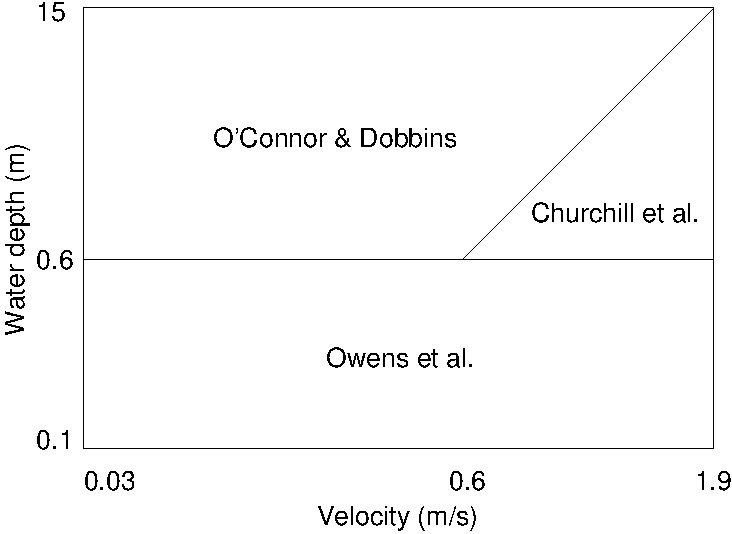
\includegraphics[width=8cm]{./graphics/validity_domain_reaeration_O2.png}\\
%  \caption{choice of the K2 formula depending on hydrodynamics of the flow}\label{k2choice}
%\end{figure}

Since these formulae are valid for a temperature of 20$^\circ$C,
the value of $k_2$ is corrected like:
\begin{equation*}
  k_2 = \left( k_2 \right)_{20^\circ C}\ \left( 1.0241 \right)^{T-20}.
\end{equation*}


The oxygen density at saturation $C_S$ can be estimated
using the temperature of water (at 20$^\circ$C, $C_S$ = 9~mg/l).
Hence if the temperature in the model is varying with time
(for example when THERMIC module is activated),
$C_S$ can be estimated with different ways using the keyword
\telkey{FORMULA FOR COMPUTING CS} (default = 0) which can have the following values:

\begin{itemize}
\item 0: constant value (default) given by
  \telkey{O2 SATURATION DENSITY OF WATER (CS)} (default = 11~mg/l),
\item 1: formula of Elmore \& Hayes,
%\[C_S = 14.652-0.41022T+0.00799T^2-7.7774.{10}^{-5}T^3\]
\item  2: formula of Montgomery.
%\[C_S = 468/(31.6+T)\]
\end{itemize}

\subsubsection{Reaeration at weirs (not used at the moment in \waqtel)}
For the O$_2$ process, a reaeration of the water due to the existence of weirs is implemented.
The water oxygen concentration is increased when crossing
from one side of a weir to the other side.
The raise of the concentration is managed through the keywords
\telkey{WEIR REAERATION COEFFICIENT RS} and \telkey{FORMULA FOR COMPUTING RS}
which can have 5 options (see \cite{El-Kadi2012} for theoretical details):

\begin{itemize}
\item 0: $RS$ is constant, in this case $RS$ is given by
  \telkey{WEIR REAERATION COEFFICIENT RS} (default 1.),
\item 1: formula of Gameson 1,
\item 2: formula of Gameson 2,
\item 3: formula of Water Research Laboratory 1,
\item 4: formula of Water Research Laboratory 2.
\end{itemize}


\section{Organic load L}

The evolution of the organic load density [L] in time is assumed
to be with a 1$^{\rm{st}}$ order law:
\begin{equation*}
 F([L]) = -k_1 [L],
\end{equation*}
where $k_1$ is a constant that describes the kinetic degradation of the organic load.
It is given using the keyword \telkey{CONSTANT OF DEGRADATION OF ORGANIC LOAD K1}
(default 0.25~d$^{-1}$).
The organic load is in mgO$_2$/l.


\section{Ammoniacal load}

The ammoniacal load $NH_4$, which is also consuming oxygen,
has a density varying in time with a 1$^{\rm{st}}$ order law given by:
\begin{equation*}
 F([NH_4]) = -k_4 [NH_4],
\end{equation*}
where $k_4$ is a nitrification kinetic constant.
It is given by \telkey{CONSTANT OF NITRIFICATION KINETIC K4} (default 0.35~d$^{-1}$).
In this module, $k_4$ is assumed to be constant and independent of remaining variables.


%\section{Final source terms}

% The oxygen density is varying under the influence of sources with respect to the following law:
%\begin{equation*}
%F\left([O_2]\right)= k_2\left(C_S-[O_2]\right)-k_1\left[L\right]-k_4\left[NH_4\right]+P-R-\frac{BEN}{h}.
%\end{equation*}
